\documentclass[11pt]{article}
\usepackage[preprint]{acl}
\usepackage{times,latexsym,graphicx,booktabs}
\usepackage[T1]{fontenc}
\usepackage[utf8]{inputenc}
\usepackage{microtype,amsmath,placeins}
\title{Reproducing ROME: Factual Model Editing\\and Robustness to Added Context}
\author{David Johnson\\University of South Florida\\CAI 5307: Natural Language Processing}
\begin{document}\maketitle\raggedbottom
\begin{abstract}
A model can learn a new answer to one question and still give its old answer when the wording changes. I compared Rank-One Model Editing (ROME) with two forms of fine-tuning on 200 CounterFact records using GPT-2 XL. ROME and ordinary fine-tuning both favored the replacement answer on all 200 direct prompts. ROME also favored it on 95.8\% of paraphrases, compared with 86.5\% for fine-tuning. On questions about related subjects, ROME favored the original answer 78.2\% of the time, compared with 42.1\% for fine-tuning. On 50 separate statements, feed-forward restoration at the last subject token peaked around layer 18. Attention restoration at the last prompt token peaked around layer 32. In the editing sample, adding 128 tokens of unrelated text lowered preference for the replacement on paraphrases by 2.0 percentage points in both the original and ROME-edited models.
\end{abstract}

\section{Introduction}
In \textit{Locating and Editing Factual Associations in GPT}, \citet{meng2022locating} asked whether a model could learn a different answer about one subject while keeping what it knew about related subjects. For example, if an edit changes the language associated with a television channel, it should carry over when someone phrases the question differently. It should also leave the model's answers about other channels intact. Testing only the sentence used to make the edit misses both possibilities.

The authors used two experiments to study this problem. First, they added noise to the part of a prompt that names the subject, then restored parts of the model's original computation to see where it recovered the expected answer. In GPT-2 XL, restoring outputs from a middle-layer feed-forward network, also called a multilayer perceptron (MLP), helped recover the answer at the end of the subject name. Restoring attention helped later, when the model was about to predict the next token. The authors then tested whether changing a middle-layer feed-forward weight matrix could change the fact that the model recalled.

ROME estimates a key for the subject by averaging its representation across different preceding texts. It then finds a value that favors the replacement answer and makes a rank-one change to map the key to that value. The update uses the second moment of the inputs to the projection, giving less weight to directions that would disrupt other commonly used keys \citep{meng2022locating}. This raises a question about the finished edit. If the model reads a paragraph before the question, does it still favor the replacement as often?

I reproduced the component traces in panels b and c of Figure~2 and the GPT-2 XL editing comparisons for four model conditions in Table~4 of \citet{meng2022locating}. I then tested the effect of adding the same unrelated passages to prompts before and after a ROME edit. The original model provides a baseline for how much the passages alone change the model's answers.

\section{Experimental setup}
\subsection{Model, cases, and editing methods}
I used GPT-2 XL, a 48-layer language model trained to predict the next token \citep{radford2019gpt2}. I shuffled the first 7,500 released CounterFact records with seed 42 and selected 200 without replacement. Each record specifies a subject, a relation, an original answer, and a replacement. All four model conditions used the same records. I scored the original model first, applied one edit, and restored the starting weights after scoring that edit. Each method therefore started from the same model for each subject. A separate 20-record pilot shared no records with the evaluation.

\begin{table}[t]\centering\small
\begin{tabular}{@{}p{.18\columnwidth}p{.75\columnwidth}@{}}\toprule
Method & Configuration \\\midrule
Original & GPT-2 XL with the original parameters.\\
FT & Layer 1 projection. Up to 25 steps, learning rate $5\times10^{-4}$.\\
FT+L & Layer 0 projection. Up to 25 steps, learning rate $5\times10^{-4}$, elementwise limit $5\times10^{-4}$.\\
ROME & Layer 17 projection, last subject token, released second moment. Value optimization up to 20 steps at a learning rate of 0.5.\\\bottomrule
\end{tabular}
\caption{GPT-2 XL settings for each method, using the released configurations \citep{romecode}. Layer numbers start at zero.}\label{tab:settings}
\end{table}

Table~\ref{tab:settings} gives the editing settings. Ordinary fine-tuning (FT) takes gradient steps on the output projection of layer 1. Constrained fine-tuning (FT+L) follows the approach of \citet{zhu2020memories} using the settings released with ROME \citep{romecode}. It edits layer 0 and limits how far each parameter can move from its starting value. ROME edits the output projection at layer 17, using the last token of the subject name to estimate its key. The two fine-tuning configurations differ in both the layer and the size of the allowed change.

\subsection{How the answers were scored}
Each record supplied one direct rewrite prompt, two paraphrases about the same subject, and ten neighborhood prompts about related subjects. For each prompt $p$, I scored the original and replacement answers separately. Equation~\ref{eq:loss} gives the mean negative log-likelihood for an answer of $m$ tokens.
\begin{equation}\label{eq:loss}
  L(a\mid p)= -\frac{1}{m}\sum_{t=1}^m \log P(a_t\mid p,a_{<t}).
\end{equation}
The model favors the candidate with the lower loss. I included the space before each answer when counting its tokens. Both answers in every sampled record were one token, so a lower loss here means a higher next-token probability. For a direct prompt or paraphrase, the edit succeeds if the replacement wins. For a neighborhood prompt, the original answer should win. A tie counts as a failure.

I averaged the prompts of each type within a record and then averaged across records. Following Meng et al., I took the harmonic mean of the three overall rates. For uncertainty intervals, I sampled the 200 records with replacement 10,000 times and used the 2.5th and 97.5th percentiles as the limits of a 95\% interval. Each draw included all prompts and model conditions for that record. This kept the comparison paired and accounted for the fact that two paraphrases of the same fact can succeed or fail together.

\section{Reproduced results}
\subsection{What changed after editing?}
\begin{figure*}[t]\centering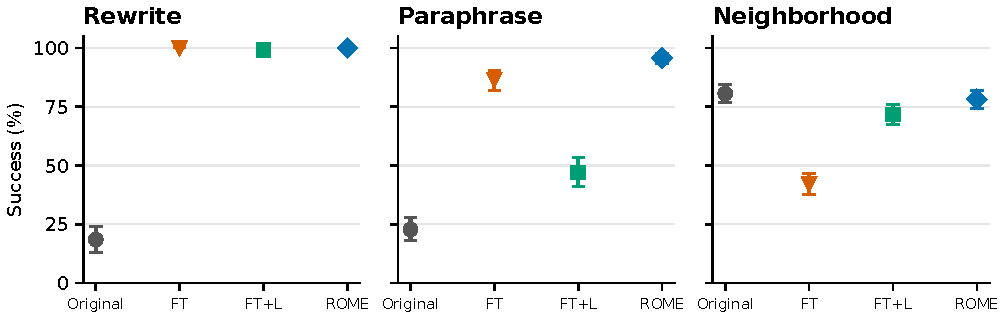
\includegraphics[width=\textwidth]{editing_scores.pdf}
\caption{Success across the three prompt groups. Points show the percentage of prompts favoring the expected candidate. Vertical bars give 95\% intervals from resampling whole records.}\label{fig:editing}
\end{figure*}
\begin{table*}[t]\centering\small\begin{tabular}{lrrrr}\toprule
Method & Efficacy & Generalization & Specificity & Harmonic mean\\\midrule
Original & 18.5 [13.0, 24.0] & 22.8 [18.0, 27.8] & 80.6 [76.8, 84.3] & 27.2 [21.4, 32.6] \\
FT & 100.0 [100.0, 100.0] & 86.5 [82.0, 90.5] & 42.1 [37.5, 46.7] & 66.2 [62.1, 69.9] \\
FT+L & 99.0 [97.5, 100.0] & 47.0 [41.0, 53.2] & 71.7 [67.3, 76.0] & 66.2 [62.0, 70.0] \\
ROME & 100.0 [100.0, 100.0] & 95.8 [93.2, 97.8] & 78.2 [74.0, 82.0] & 90.3 [88.3, 92.0] \\
\bottomrule\end{tabular}
\caption{Editing scores on the 200 CounterFact records. Efficacy, generalization, and specificity are the success rates (\%) for rewrites, paraphrases, and neighborhood prompts, respectively. Brackets give 95\% paired bootstrap intervals.}\label{tab:rates}
\end{table*}
Both ROME and ordinary fine-tuning favored the replacement on all 200 direct prompts. The difference showed up when the question changed. ROME favored the replacement on 383 of 400 paraphrases, compared with 346 for FT. On the 2,000 neighborhood prompts, ROME favored the original answer on 1,563 and FT on 842. That gives ROME an advantage of about 36 percentage points on related subjects (95\% paired interval, 31.9 to 40.3). Figure~\ref{fig:editing} shows this difference alongside the direct-prompt and paraphrase results. Table~\ref{tab:rates} gives the rates and intervals for all four conditions.

FT+L favored the original answer on 71.7\% of neighborhood prompts, between FT (42.1\%) and ROME (78.2\%). The replacement won on 188 of 400 paraphrases (47.0\%). FT and FT+L ended up with nearly identical harmonic means of 66.2 even though their errors fell on different prompts. Table~\ref{tab:counts} shows the counts behind those scores.
\begin{table}[t]\centering\small
\begin{tabular}{@{}lrrr@{}}\toprule
Method & Rewrite & Paraphrase & Neighborhood \\\midrule
Original & 37 & 91 & 1,612 \\
FT & 200 & 346 & 842 \\
FT+L & 198 & 188 & 1,434 \\
ROME & 200 & 383 & 1,563 \\\bottomrule
\end{tabular}
\caption{Prompt counts behind Table~\ref{tab:rates}. There were 200 rewrites, 400 paraphrases, and 2,000 neighborhood prompts.}\label{tab:counts}
\end{table}

The original model itself favored the original answer on 1,612 of the 2,000 neighborhood prompts. Looking just at those 1,612 gives a more direct measure of how often an edit kept a preference the model already had. ROME kept 1,562 (96.9\%) and FT kept 836 (51.9\%). Across all related prompts, the original model still had slightly higher specificity than ROME (80.6\% versus 78.2\%).

\subsection{When the direct edit worked but the paraphrases failed}
ROME favored the replacement on both paraphrases for 186 records, compared with 164 for FT. In three cases, ROME succeeded on the direct rewrite and favored the original answer on both paraphrases. The subjects were CGTN Spanish, Double-Time Records, and the United Nations. Table~\ref{tab:failures} shows how the result changed across the three wordings for CGTN Spanish.

\begin{table*}[t]\centering\small
\begin{tabular}{@{}p{.55\textwidth}rrl@{}}\toprule
Prompt or prompt ending & Korean & Spanish & Preferred answer\\\midrule
The language of CGTN Spanish was & 0.06 & 7.65 & Korean\\
Paraphrase 1, ending in \textit{CGTN Spanish is written in} & 6.72 & 2.77 & Spanish\\
Paraphrase 2, ending in \textit{CGTN Spanish was written in} & 7.44 & 2.73 & Spanish\\\bottomrule
\end{tabular}
\caption{Candidate losses after editing CGTN Spanish from Spanish to Korean. Lower values indicate a higher probability. The paraphrases are identified by their endings.}\label{tab:failures}
\end{table*}

On the direct prompt, the model strongly favored Korean. Both paraphrases added a different lead-in and asked what language the channel was written in. In both cases the model favored Spanish. A similar pattern occurred for Double-Time Records. The direct edit favored opera over jazz, but both paraphrases favored jazz. On one paraphrase the losses were close (8.96 for opera and 8.57 for jazz). By the binary scoring rule, that counts the same as the larger reversals for CGTN Spanish. Neither score says which word the model would generate from its full vocabulary.

\subsection{Comparison with the published benchmark}
\begin{table}[t]\centering\small\begin{tabular}{lrrrr}\toprule
Method & Eff. & Gen. & Spec. & Mean\\\midrule
Original & 22.2 & 24.7 & 78.1 & 30.5 \\
FT & 100.0 & 87.9 & 40.4 & 65.1 \\
FT+L & 99.1 & 48.7 & 70.3 & 66.9 \\
ROME & 100.0 & 96.4 & 75.4 & 89.2 \\
\bottomrule\end{tabular}\caption{GPT-2 XL results on 7,500 CounterFact records from Table~4 of \citet{meng2022locating}. The final column is the harmonic mean of the three success rates.}\label{tab:published}
\end{table}
Table~\ref{tab:published} shows the corresponding values from Meng et al.'s Table~4. In their 7,500-record test, ROME's specificity was 35.0 points higher than FT's. In this 200-record subset it was about 36 points higher. ROME's harmonic mean was also close to the published result (90.3 versus 89.2). Both samples show why testing on related subjects matters: the two methods look equally successful if the only measure is the direct rewrite.

The largest difference for the original model was on direct rewrites. It favored the replacement on 18.5\% here and 22.2\% in the published results. On paraphrases those rates were 22.8\% and 24.7\%. The two studies used records from the same evaluation pool. Comparing their means shows how well the published pattern carries over to the smaller sample. Within my sample I could also pair each method with ROME on the same facts (Table~\ref{tab:paired}). Relative to FT+L, ROME gained about 49 points on paraphrases and six points on neighborhood prompts. Relative to the original model, ROME's neighborhood score fell by about 2.5 points. An edit can therefore score well against the fine-tuning baselines and still cost the model some of its preferences for the original answer on related facts.

\begin{table*}[t]\centering\small
\begin{tabular}{@{}lrrr@{}}\toprule
Comparison & Rewrite & Paraphrase & Neighborhood\\\midrule
ROME minus original & 81.5 [76.0, 87.0] & 73.0 [67.8, 78.0] & $-2.5$ [$-3.9$, $-1.3$]\\
ROME minus FT & 0.0 [0.0, 0.0] & 9.2 [5.0, 13.8] & 36.0 [31.9, 40.3]\\
ROME minus FT+L & 1.0 [0.0, 2.5] & 48.8 [42.8, 54.8] & 6.5 [3.6, 9.5]\\\bottomrule
\end{tabular}
\caption{Paired differences in percentage points across the same 200 records, with 95\% bootstrap intervals. Differences were calculated before rounding.}\label{tab:paired}
\end{table*}

\subsection{Tracing a factual prediction}
I used the original GPT-2 XL model to trace predictions on a separate collection of factual statements. Its top next token matched the expected answer on 1,208 of 1,209 statements after trimming whitespace. I randomly selected 50 from those matches. This lets me follow the probability of an answer the model already predicts, from the point where it reads the subject name to the point where it gives its answer.

For each statement, I added Gaussian noise to the embeddings of the subject tokens. The noise had three times the standard deviation of the subject-token embeddings in the released collection. I averaged the answer probabilities over ten noise draws. I then restored either the clean MLP output or the clean attention output at one token position. Each restoration covered up to ten consecutive layers. The window was shorter near the first and last layers.

\begin{figure*}[t]\centering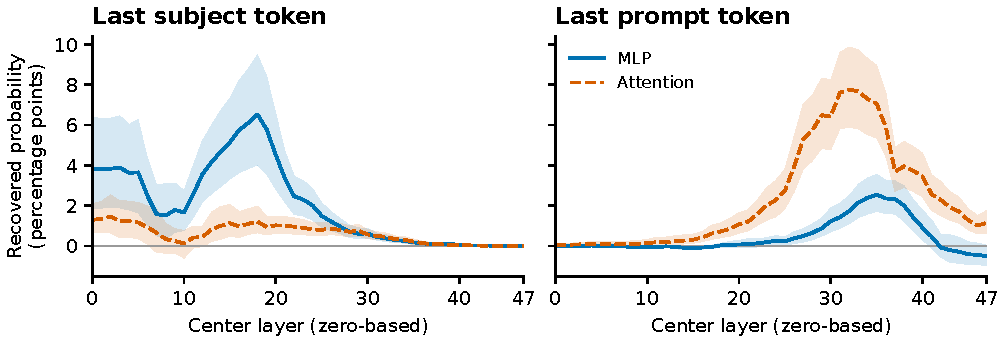
\includegraphics[width=\textwidth]{tracing_profiles.pdf}
\caption{Mean recovery in the expected token probability after restoring MLP outputs (solid blue) or attention outputs (dashed orange). Panels show the last subject token and the last prompt token. Shading gives pointwise 95\% intervals across the 50 statements.}\label{fig:profiles}
\end{figure*}
\begin{figure*}[t]\centering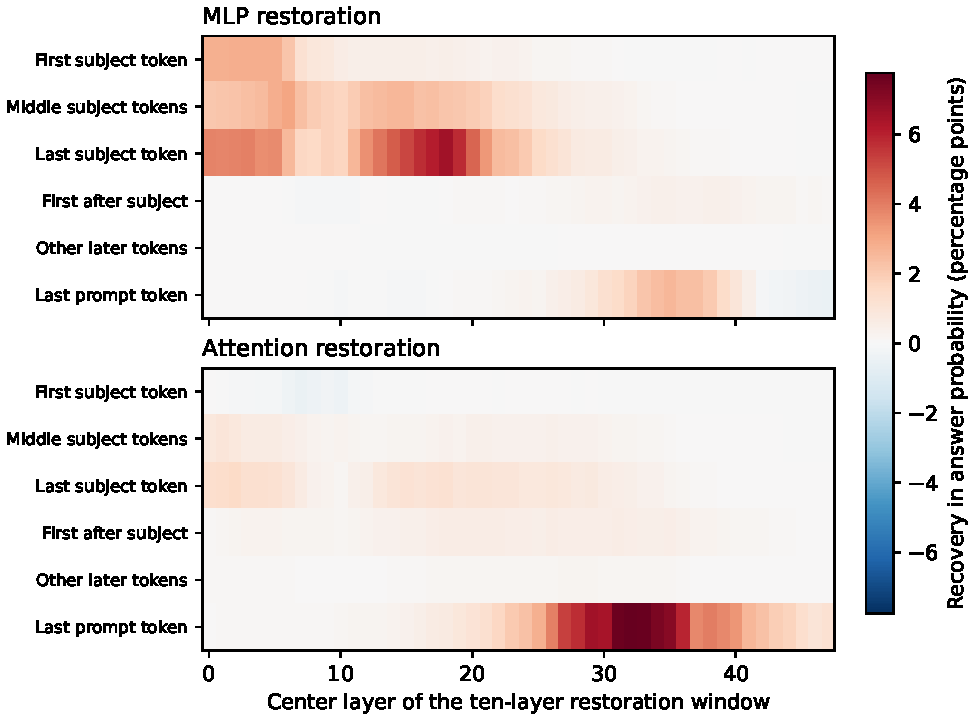
\includegraphics[width=.95\textwidth]{tracing.pdf}\caption{Mean recovery by token position and layer. Red indicates that restoration raised the expected answer probability relative to adding noise alone. Blue indicates that it fell. Both panels use the same scale.}\label{fig:heat}
\end{figure*}

For each statement, I subtracted the probability under corruption from the probability after restoration. The average of those differences is the average indirect effect in the terminology of \citet{meng2022locating}. Figure~\ref{fig:profiles} compares the two positions highlighted in the paper. Every statement contributes one final subject token and one final prompt token. The shaded intervals come from resampling the 50 statements and taking the middle 95\% of the estimated effects at each layer.

At the last subject token, MLP recovery peaked at 6.5 points for the window centered at layer 18. Meng et al. found 6.6 points around layer 17 across 1,000 statements. At the last prompt token, attention recovery peaked at 7.8 points around layer 32, close to their roughly 8.0 points at the same layer. Both samples put the MLP peak at the subject name in the middle layers and the attention peak just before the model predicted the answer. The nearby window centers cover many of the same layers. The size of the initial disruption did differ between studies. Meng et al. reported a drop from 27.0\% to 8.5\% when they added noise. The drop on my 50 statements was from 25.1\% to 3.1\%. Comparing gains from each study's own corrupted baseline accounts for their different starting probabilities.

Figure~\ref{fig:heat} shows the other token positions. For middle positions I first averaged tokens within a statement so that a longer name could not outweigh a shorter one. Forty-one statements had middle subject tokens and 45 had tokens between the first and last positions after the subject. The authors' heat map pools the middle tokens across statements and subtracts the overall mean under corruption \citep{romecode}. At layer 6, for example, middle-subject MLP recovery on these same statements is 3.1 points with my average and 0.6 points with theirs. Each statement contributes exactly one token to each of the last-subject and last-prompt curves, so those curves are the same under either calculation.

\paragraph{An example from the tracing sample.}
For a prompt about Vita Semerenko's citizenship, GPT-2 XL assigned a 19.8\% probability to the answer token for Ukraine. Adding noise to her name lowered it to 3.1\%. Restoring MLP outputs at the last token of her name around layer 18 raised the probability to 9.2\%. In a separate pass, restoring attention at the final prompt token around layer 32 raised it to 10.2\%. Each restoration recovered part of the prediction during that pass. ROME updates the middle-layer MLP weights. That change also affects later prompts about the subject and its neighbors.

\FloatBarrier
\section{Extension results: adding unrelated text}
ROME uses several preceding texts to estimate a subject key when making an edit. I tested a related question at prediction time: how much does adding an unrelated paragraph change the model's preference on a question about the edited subject or a nearby fact? I compared the original model with ROME on the same 200 records. I added passages only to paraphrases and neighborhood prompts. These test whether the edit carries over to a new wording and whether related facts change. Comparing ROME with the original model measures the extra sensitivity associated with editing.

\subsection{Passages and comparisons}
I used two descriptions, one of a sheet of paper beside a tray and one of a row of tiles on a ledge. I took the first 32 or 128 GPT-2 tokens of each passage, followed them with two newlines, and left the original question and the two answers unchanged. Neither passage contained a sampled subject name or candidate answer in a case-insensitive whole-word match. Both lengths came from the same passages, and the token cutoffs leave some sentences unfinished. Appendix~\ref{app:passages} gives the exact text.

For each model and prefix length, I scored both passages on the two paraphrases and ten neighborhood prompts for every record. That gives 4,800 prefixed comparisons per model at each length. All inputs fit within the model's 1,024-token context window. I averaged the two passages at each length within each record, then subtracted its score without a prefix. To test whether editing changed sensitivity, I subtracted the original model's change from ROME's change on the same record. The uncertainty intervals use the same paired resampling as the editing comparison. Because all records saw the same two passages, the intervals describe variation across facts.

\begin{table*}[t]\centering\small\begin{tabular}{rlrr}\toprule
Prefix tokens & Comparison & Paraphrase change & Neighborhood change\\\midrule
32 & Original & -1.8 [-4.4, +0.8] & -1.0 [-2.4, +0.4] \\
32 & ROME & -0.4 [-1.8, +1.0] & -0.8 [-2.3, +0.8] \\
32 & ROME minus original & +1.4 [-1.5, +4.2] & +0.2 [-0.4, +0.9] \\
128 & Original & -2.0 [-4.9, +0.8] & -2.3 [-4.0, -0.8] \\
128 & ROME & -2.0 [-3.9, -0.4] & -1.7 [-3.4, -0.1] \\
128 & ROME minus original & 0.0 [-3.4, +3.4] & +0.6 [-0.1, +1.4] \\
\bottomrule\end{tabular}\caption{Change in candidate preference after adding a passage, in percentage points. The expected candidate is the replacement for paraphrases and the original answer for neighborhood prompts. Brackets give 95\% paired bootstrap intervals.}\label{tab:prefix}
\end{table*}

\subsection{Did the edit change sensitivity to the passages?}
Without a prefix, ROME favored the replacement on 95.8\% of paraphrases and the original model did so on 22.8\%. With the 128-token passages, both rates fell by 2.0 percentage points. For ROME that meant the edit carried over to fewer paraphrases. For the original model it meant choosing the counterfactual replacement less often. The difference between the two changes was 0.0 points (95\% paired interval, $-3.4$ to $+3.4$). Table~\ref{tab:prefix} shows the shorter passages and the neighborhood results alongside this comparison.

On neighborhood prompts, the longer passages lowered preference for the original answer by 2.3 points in the original model and 1.7 in ROME. Here a lower rate has the same meaning for both models because the prompt asks about a different subject. The difference between the changes was 0.6 points, with an interval from $-0.1$ to $+1.4$. Both models became less likely to favor the original answer. The interval leaves open whether the drop differed between models.

\subsection{Which preferences changed?}
The same two-point drop on paraphrases came from different sets of answers changing direction. Each model saw 400 paraphrases with two passages, for 800 comparisons at each prefix length. With 128 tokens, the original model lost 43 preferences for the replacement and gained 27. ROME lost 22 and gained six. Each model ended up with 16 fewer replacement preferences out of 800, even though the original model changed its preference on 70 comparisons and ROME on 28.

Table~\ref{tab:switches} gives both directions for paraphrases and neighborhood prompts. On neighborhood prompts, a loss means the model switched to the replacement on a question about a different subject. At 128 tokens, ROME lost 205 original-answer preferences and gained 137 across 4,000 comparisons. That net loss of 68 gives the 1.7-point decline in Table~\ref{tab:prefix}. The models started with very different paraphrase preferences, so a smaller number of switches need not mean that ROME was more robust.

\begin{table}[t]\centering\small
\begin{tabular}{@{}llrrrr@{}}\toprule
& & \multicolumn{2}{c}{Paraphrases} & \multicolumn{2}{c}{Neighbors}\\
Tokens & Model & Lost & Gained & Lost & Gained\\\midrule
32 & Original & 40 & 26 & 167 & 126\\
32 & ROME & 11 & 8 & 175 & 144\\
128 & Original & 43 & 27 & 211 & 118\\
128 & ROME & 22 & 6 & 205 & 137\\\bottomrule
\end{tabular}
\caption{Changes in the preferred candidate after adding a passage. A loss means the expected candidate won without the passage and lost with it. A gain is the reverse. Each row covers 800 paraphrase and 4,000 neighborhood comparisons.}\label{tab:switches}
\end{table}

\FloatBarrier
\section{Resources}
I used an NVIDIA Tesla T4 in Google Colab with GPT-2 XL in 32-bit floating point. The 200 editing cases took 2.38 hours on the GPU and used up to 9.58 GB of GPU memory.

\section{Code}
The repository includes the Colab notebook, the saved candidate scores and traces, and the scripts for recalculating the results and drawing the figures on a CPU. The README gives instructions for running either the full experiment or the analysis of the saved results.

\noindent\url{https://github.com/Davids-AIresearch-USF/rome-gpt2-xl-reproduction}

\section{Conclusion}
Both ROME and ordinary fine-tuning favored the replacement on all 200 direct rewrites. In 163 cases that reversed the original model's preference. ROME transferred to more paraphrases and kept more of the original model's preferences on related subjects. Three ROME edits still failed on both paraphrases. In the tracing sample, MLP restoration helped at the subject name and later attention restoration helped at the end of the prompt, as Meng et al. found. Adding unrelated text had a much smaller effect on the editing results: the longer passages shifted paraphrase preference by the same two points before and after editing.

\FloatBarrier
\bibliography{references}

\clearpage
\appendix
\section{Text added before the prompts}\label{app:passages}
Each passage below contains the full 128-token prefix. Bold type marks the first 32 tokens, which were also tested on their own. Both versions were followed by a blank line before the question.

\paragraph{Sheet and tray.} \textbf{A folded sheet rested beside a shallow tray on a plain surface. The smallest crease ran from one corner toward the middle. Along the far edge a darker band} shaded the paper. A small wooden bead rested in the tray. Its shadow reached just past a faint scratch. Beneath the sheet, a narrow strip of cloth lay flat. The weave was tighter near the edge and looser where the cloth had been folded. Light shifted across the surface while the objects stayed still. A faint ring marked the spot where a second tray had rested. The paper curled slightly at one corner, leaving a small gap above the cloth. From the side

\paragraph{Tiles and brush.} \textbf{A short row of tiles lined a narrow ledge. Each tile had a rough underside and a smooth face. A soft brush rested across the gap between two of them}. Its bristles spread slightly where they touched the ledge. Near the handle a loose thread hung over the edge. A faint stripe crossed the middle tile and curved toward one corner. A smaller stripe stopped beside it. Seen from above, the pair looked almost parallel. The surface beneath the ledge had a shallow groove that filled with dust along one side. A small patch remained clear under the brush. Where the light struck the groove, its edge cast a narrow shadow. A speck
\end{document}
